\section{Асимметричные протоколы}
\selectlanguage{russian}

Асимметричные протоколы, или же протоколы, основанные на криптосистемах с открытыми ключами, позволяют ослабить требования к предварительному этапу протоколов. Вместо общего секретного ключа, который должны иметь две стороны (либо каждая из сторон и доверенный центр), в рассматриваемых ниже протоколах стороны должны предварительно обменяться открытыми ключами (между собой либо с доверенным центром). Такой предварительный обмен может проходить по открытому каналу связи, в предположении, что криптоаналитик не может повлиять на содержимое канала связи на данном этапе.

\subsection{Протокол Диффи~---~Хеллмана}\index{протокол!Диффи~---~Хеллмана}\label{section-protocols-diffie-hellman}
\selectlanguage{russian}

Первый алгоритм с открытым ключом был предложен Диффи и Хеллманом в работе 1976 года <<Новые направления в криптографии>> (\langen{Bailey Whitfield Diffie, Martin Edward Hellman, ``New directions in cryptography''},~\cite{Diffie:Hellman:1976}). Данный протокол, который также можно назвать \emph{схемой Диффи~---~Хеллмана}, стал первым, позволивший уменьшить требования к каналу связи для установления защищённого соединения без предварительного обмена ключами.

Протокол позволяет двум сторонам создать общий сеансовый ключ используя такой канал связи, который может прослушивать злоумышленник, но в предположении, что последний не может менять содержимое сообщений.

Пусть $p$ -- большое простое число\index{число!простое}, $g$ -- примитивный элемент группы $\Z_p^*$, ~ $y = g^x \bmod p$, причём $p, y, g$ известны заранее. Функцию $y=g^{x} \bmod p$ считаем однонаправленной, то есть вычисление функции при известном значении аргумента является лёгкой задачей, а её обращение (нахождение аргумента) при известном значении функции -- трудной.\footnote{Обратную функцию $x = \log_g y \bmod p$ называют функцией дискретного логарифма. В настоящий момент не существует быстрых способов вычисления такой функции для больших простых $p$.}

Протокол обмена состоит из следующих действий.

\begin{figure}
    \centering
    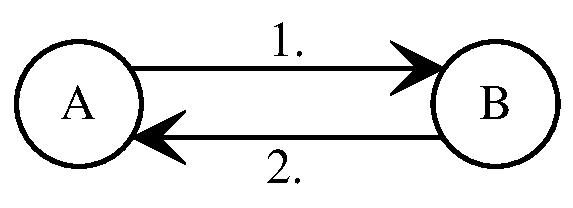
\includegraphics[width=0.5\textwidth]{pic/key_distribution-diffie-hellman}
    \caption{Общая схема взаимодействия участников в протоколе Диффи~---~Хеллмана\label{fig:key_distribution-diffie-hellman}}
\end{figure}

\begin{protocol}
    \item[(1)] Алиса выбирает случайное $2 \leq a \leq p - 1$
    \item[{}] $Alice \to \left\{ A = g ^ a \bmod p \right\} \to Bob$
    \item[(2)] Боб выбирает случайное $2 \leq b \leq p-1$
    \item[{}] Боб вычисляет сеансовый ключ $K = A ^ b \bmod p$
    \item[{}] $Bob \to \left\{ B = g ^ b \bmod p \right\} \to Alice$
    \item[(3)] Алиса вычисляет $K = B ^ a \bmod p$
\end{protocol}

Таким способом создан общий секретный сеансовый ключ $K$. За счёт случайного выбора значений $a$ и $b$ в новом сеансе будет получен новой сеансовый ключ.

Протокол обеспечивает только генерацию новых сеансовых ключей (цель G10). В отсутствие третей доверенной стороны он не обеспечивает ни аутентификацию сторон (цель G1), из-за отсутствия проходов с подтверждением владения ключом отсутствует аутентификация ключа (цель G8). Зато, так как протокол не использует длительные <<мастер>>-ключи, можно говорить о том, что он обладает свойством совершенной прямой секретности (цель G9).

Протокол можно использовать только с такими каналами связи, в которые не может вмешаться активный криптоаналитик. В противном случае протокол становится уязвим к простой <<атаке посередине>>.

\begin{figure}
    \centering
    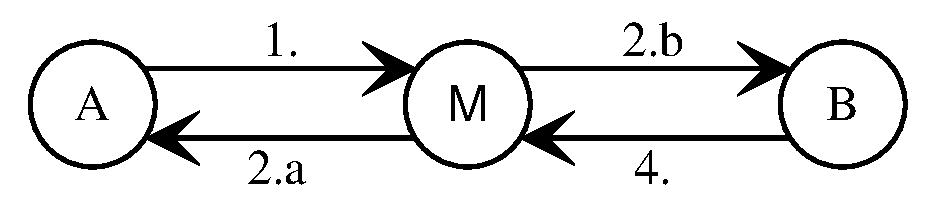
\includegraphics[width=0.67\textwidth]{pic/key_distribution-diffie-hellman-mitm}
    \caption{Схема взаимодействия участников в протоколе Диффи~---~Хеллмана в модели с активным криптоаналитиком\label{fig:key_distribution-diffie-hellman-mitm}}
\end{figure}

\begin{protocol}
    \item[(1)] Алиса выбирает случайное $2 \leq a \leq p - 1$
    \item[{}] $Alice \to \left\{ A = g ^ a \bmod p \right\} \to Mellory~(Bob)$
    \item[(2)] Меллори выбирает случайное $2 \leq m \leq p-1$
    \item[{}] Меллори вычисляет сеансовый ключ для канала с Алисой
        \[K_{AM} = A ^ m \bmod p = g ^ {am} \bmod p\]
    \item[{}] $Mellory~(Alice) \to \left\{ M = g ^ m \bmod p \right\} \to Bob$
    \item[{}] $Mellory~(Bob) \to \left\{ M = g ^ m \bmod p \right\} \to Alice$
    \item[(3)] Алиса вычисляет сеансовый ключ для канала с Меллори (думая, что Меллори это Боб)
        \[K_{AM} = M ^ a \bmod p = g ^ { am } \bmod p\]
    \item[(4)] Боб выбирает случайное $2 \leq b \leq p-1$
    \item[{}] Боб вычисляет сеансовый ключ для канала с Меллори (думая, что Меллори это Алиса)
        \[K_{BM} = M ^ b \bmod p = g ^ { bm } \bmod p\]
    \item[{}] $Bob \to \left\{ B = g ^ b \bmod p \right\} \to Mellory~(Alice)$
    \item[(5)] Меллори вычисляет сеансовый ключ для канала с Бобом
        \[K_{BM} = B ^ m \bmod p = g ^ { bm } \bmod p\]
\end{protocol}

В результате Алиса и Боб получили новые сеансовые ключи, но <<защищённый>> канал связи установили не с друг с другом, а со злоумышленником, который теперь имеет возможность ретранслировать или изменять все передаваемые сообщения между Алисой и Бобом.

Протокол Диффи~---~Хеллмана отличается от большей части протоколов распространения ключей из-за того, что не использует другие криптографические примитивы (функции шифрования, электронно-цифровой подписи или хеширования), но сам по себе является в некотором смысле криптографическим примитивом для построения более сложных протоколов. Он обеспечивает генерацию случайного числа в распределённой системе без доверенного центра. Причём ни одна из сторон не может заставить другую сторону использовать старый сессионный ключ, в отличие от, например, протокола Yahalom\index{протокол!Yahalom} из раздела~\ref{section-protocols-yahalom}.

Протокол можно изменить таким образом, чтобы вместо мультипликативной группы простого умножения использовать аддитивную группу сложения точек эллиптической кривой (см. раздел~\ref{section-math-ec-groups}). В этом случае стороны по прежнему будут выбирать некоторые случайные целые числа, но не возводить генератор-число в степень, а умножать генератор-точку на загаданное число.

\begin{protocol}
    \item[(0)] Стороны договорились о группе точек эллиптической кривой $\group{E}$, её циклической подгруппе $\group{G}$ мощности $n = \| \group{G} \|$ и генераторе $G$ группы $\group{G}$ (или хотя бы достаточно большой подгруппы группы $\group{G}$).
    \item[(1)] Алиса выбирает случайное $2 \leq a \leq n - 1$
    \item[{}] $Alice \to \left\{ A = a \times G \right\} \to Bob$
    \item[(2)] Боб выбирает случайное $2 \leq b \leq n - 1$
    \item[{}] Боб вычисляет точку $K = b \times A$
    \item[{}] $Bob \to \left\{ B = g \times G \right\} \to Alice$
    \item[(3)] Алиса вычисляет точку $K = a \times B$
\end{protocol}

В качестве нового сессионного ключа стороны могут выбрать, например, первую координату найденной точки $K$.


%\section{Протоколы с аутентификацией}

\subsection{Односторонняя аутентификация}

\section{Системы Эль-Гамаля}
\selectlanguage{russian}

\subsection[Шифрование]{Система шифрования Эль-Гамаля}

Эта система шифрования с открытым ключом опубликована Эль-Гамалем (El-Gamal) в 1985 году. Рассмотрим принципы ее построения.

Пусть имеется мультипликативная группа $\Z_p^* = \{1, 2, \dots, p-1\}$, где $p$ -- большое простое число, содержащее 1024 двоичных разряда. Существует целое число $g$, называемое примитивным элементом, который порождает все ненулевые числа группы, причем $1 < g < p-1$.

    \[ g\mod p, ~~ g^2\mod p, ~~ \dots, ~~ g^{p-1} = 1\mod p \]

Выберем целое число $x$ в интервале $1 \le x \le p-1$. Вычислим
    \[ y = g^x \mod p. \]
Известно, что в конечном поле функция $y(x)$ -- вычислительно однонаправленная.

Задачей \textbf{дискретного логарифмирования}\index{задача!дискретного логарифмирования} в мультипликативной группе $\Gr$ называется нахождение $x$ по заданным элементам $a,b \in \Gr, ~ b = a^x$. Для групп большого размера $2^{150}$--$2^{1000}$ при выборе элемента $a$ генератором группы или подгруппы большого порядка дискретный логарифм известными алгоритмами не вычислим за доступное время, все известные алгоритмы -- неполиномиальные.

Процедура шифрования криптосистемы  Эль-Гамаля состоит из следующих операций.

\begin{enumerate}
    \item \textbf{Создание пары из секретного и открытого ключей стороной $A$.}
        \begin{enumerate}
            \item $A$ выбирает простое случайное число $p$.
            \item Выбирает генератор $g$ (в программных реализациях алгоритма генератор часто выбирается малым числом, например $g = 2 \mod p$).
            \item Выбирает $x \in [1, p-1]$ с помощью генератора случайных чисел.
            \item Вычисляет $y=g^{x}\mod p$,
            \item Создает секретный и открытые ключи $\SK$ и $\PK$:
                \[ \SK = (x), ~ \PK = (p, g, y). \]
                Криптостойкость задается битовой длиной параметра $p$.
        \end{enumerate}
    \item \textbf{Шифрование на открытом ключе стороной $B$.}
        \begin{enumerate}
            \item $B$ извлекает открытый ключ $\text{PK} = (p, g, y)$ из директории стороны $A$.
            \item Сообщение представляется числом $m \in [1,p-1]$.
            \item Выбирает случайное число $r \in [1, p-1]$ и вычисляет
                \[ \begin{array}{l}
                    a = g^r \mod p, \\
                    b = m y^r \mod p.
                \end{array} \]
            \item Создает шифрованное сообщение в виде
                \[ c = (a,b) \]
                и посылает стороне $A$.
        \end{enumerate}
    \item \textbf{Расшифрование на секретном ключе стороной $A$.}
        \begin{enumerate}
            \item Используя секретный ключ $x$, $A$ вычисляет
                \[ m = \frac{b}{a^x} \mod p. \]
            \item Расшифрование корректно, так как
                \[ \begin{array}{l}
                    \frac{b}{a^x} = \frac{m y^r}{g^{rx}} = m \mod p, \\
                    m \mod p \equiv m.
                \end{array} \]
        \end{enumerate}
\end{enumerate}


\subsubsection{Пример системы}

\begin{enumerate}
    \item Генерирование параметров.
        \begin{enumerate}
            \item Выберем $p=41$.
            \item Группа $\Z_p^*$ циклическая, найдем генератор (примитивный элемент). Порядок группы
                \[ |\Z_p^*| = \phi(p) = p-1 = 40. \]
                Делители 40: 2, 4, 5, 8, 10, 20. Элемент группы является примитивным, если все его степени, соответствующие делителям порядка группы, не сравнимы с 1. Из табл. \ref{tab:elgamal-generator-search} видно, что число $g = 6$ является генератором всей группы.
                \begin{table}[h!]
                    \centering
                    \caption{Поиск генератора в циклической группе $\Z_{41}^*$. Элемент 6 -- генератор\label{tab:elgamal-generator-search}}
                    \resizebox{\textwidth}{!}{ \begin{tabular}{|c|c|c|c|c|c|c|c|c|}
                        \hline
                        \multirow{2}{*}{Элемент} & \multicolumn{7}{|c|}{Степени} & \multirow{2}{*}{Порядок элемента} \\
                        \cline{2-8}
                                & 2   & 4   & 5   & 8  & 10 & 20 & 40 & \\
                        \hline
                        2       & 4   & 16  & -9  & 10 & -1 & 1  &    & 20 \\
                        3       & 9   & -1  & -3  & 1  &    &    &    & 8 \\
                        5       & -16 & 10  & 9   & 18 & -1 & 1  &    & 20 \\
                        6       & -5  & -16 & -14 & 10 & -9 & -1 & 1  & 40 \\
                        \hline
                    \end{tabular} }
                \end{table}
            \item Выберем случайное $x = 19 \in [1, p-1]$.
            \item Вычислим
                \[ \begin{array}{ll}
                    y & = g^x \mod p = \\
                    & = 6^{19} \mod 41 = \\
                    & = 6^{1 + 2 + 4 \cdot 0 + 8 \cdot 0 + 16} \mod 41 = \\
                    & = 6^1 \cdot 6^2 \cdot 6^{4 \cdot 0} \cdot 6^{8 \cdot 0} \cdot 6^{16} \mod 41 = \\
                    & = 6 \cdot (-5) \cdot (-16)^0 \cdot 10^0 \cdot 18 \mod 41 = \\
                    & = -7 \mod 41.
                \end{array} \]
            \item Открытый и секретные ключи:
                \[ \PK = (p:41, g:6, y:-7), ~ \SK = (x:19). \]
        \end{enumerate}
    \item Шифрование.
        \begin{enumerate}
            \item Пусть сообщением является число $m = 3 \in \Z_p^*$.
            \item Выберем случайное число $r = 25 \in [1, p-1]$.
            \item Вычислим
                \[ \begin{array}{l}
                    a = g^r \mod p = 6^{25} \mod 41 = 14 \mod 41, \\
                    b = m y^r \mod p = 3 \cdot (-7)^{25} \mod 41 = -9 \mod 41.
                \end{array} \]
            \item Шифротекстом является пара чисел
                \[ c = (a:14, ~ b:-9). \]
        \end{enumerate}
    \item Расшифрование.
        \begin{enumerate}
            \item Пусть получен шифротекст
                \[ c = (a:14, ~ b:-9). \]
            \item Вычислим открытый текст как
                \[ \begin{array}{ll}
                    m & = \frac{b}{a^x} \mod p = \\
                    & = -9 \cdot (14^{-1})^{19} \mod 41 = \\
                    & = -9 \cdot 3^{19} \mod 41 = \\
                    & = -9 \cdot (-14) \mod 41 = \\
                    & = 3 \mod 41. \\
                \end{array} \]
        \end{enumerate}
\end{enumerate}


\subsection[Электронная цифровая подпись]{Электронная цифровая подпись \protect\\ Эль-Гамаля}

Криптосистема Эль-Гамаля, как и криптосистема RSA,  может быть использована для создания ЭЦП.

По-прежнему имеются два пользователя $A$ и $B$ и незащищенный канал связи между ними. Пользователь $A$  хочет подписать свое открытое сообщение $m$  для того, чтобы пользователь $B$ мог убедиться, что именно $A$ подписал сообщение.

Пусть $A$ имеет секретный ключ $\SK = (x)$, открытый ключ $\PK = (p,g,y)$ (полученные так же, как и в системе шифрования Эль-Гамаля) и хочет подписать открытое сообщение. Обозначим подпись $S(m)$.

Для создания подписи $S(m)$ пользователь $A$ выполняет следующие операции:
\begin{itemize}
    \item вычисляет значение криптографической хэш-функции  $h(m) \in [0,p-2]$, от своего открытого сообщения $m$;
    \item выбирает случайное число $r, ~ \gcd(r, p-1)=1$;
    \item используя открытый ключ, вычисляет
        \[ \begin{array}{l}
            a = g^r \mod p, \\
            b = \frac{h(m) - xa}{r} \mod (p-1); \\
        \end{array} \]
    \item создает подпись в виде двух чисел
        \[ S(m) = (a, b) \]
        и посылает сообщение с подписью $(m, S(m))$.
\end{itemize}

Получив сообщение,  $B$ осуществляет проверку подписи, выполняя следующие операции:
\begin{itemize}
    \item по известному сообщению $m$ вычисляет значение хэш-функции $h(m)$;
    \item вычисляет
        \[ \begin{array}{l}
            f_1 = g^{h(m)} \mod p, \\
            f_2 = y^a a^b \mod p; \\
        \end{array} \]
    \item сравнивает значения $f_1$ и $f_2$, если
        \[ f_1 = f_2, \]
        то подпись подлинная, в противном случае -- фальсифицированная (или случайно испорченная).
\end{itemize}

Покажем, что проверка подписи корректна. По малой теореме Ферма получаем
\[ \begin{array}{ll}
    f_1 & = g^{h(m)} \mod p = \\
    & \\
    & = g^{h(m) \mod (p-1)} \mod p; \\
\end{array} \] \[ \begin{array}{ll}
    f_2 & = y^a a^b \mod p = \\
    & = \underbrace{\left( g^x \right)^a}_{y^a} \cdot
        \underbrace{\left( g^r \mod p \right)^{\frac{h(m) - xa}{r} \mod (p-1)}}_{a^b} \mod p = \\
    & \\
    & = g^{xa \mod (p-1)} ~\cdot~ g^{h(m) - xa \mod (p-1)} \mod p = \\
    & = g^{h(m) \mod (p-1)} \mod p = \\
    & = f_1.
\end{array} \]

\subsubsection{Пример системы}

\begin{enumerate}
    \item Генерирование параметров.
        \begin{enumerate}
            \item Выберем $p=41$.
            \item Выберем генератор $g=6$ в группе $\Z_{41}^*$.
            \item Выберем случайное $x = 19 \in [1, p-1]$.%, ~ \gcd(x, p-1) = 1$.
            \item Вычислим
                \[ \begin{array}{ll}
                    y & = g^x \mod p = \\
                    & = 6^{19} \mod 41 = \\
                    & = 6^{1 + 2 + 4 \cdot 0 + 8 \cdot 0 + 16} \mod 41 = \\
                    & = 6 \cdot (-5) \cdot (-16)^0 \cdot 10^0 \cdot 18 \mod 41 = \\
                    & = -7 \mod 41. \\
                \end{array} \]
            \item Открытый и секретные ключи:
                \[ \PK = (p:41, g:6, y:-7), ~ \SK = (x:19). \]
        \end{enumerate}
    \item Подписание.
        \begin{enumerate}
            \item От сообщения $m$ вычисляется хэш $h = H(m)$. Пусть хэш $h  = 3 \in [0, p-2]$.
            \item Выберем случайное $r = 9 \in [1, p-2]$: \\
                $\gcd(r=9, p-1 = 40) = 1$.
            \item Вычислим
                \[ \begin{array}{ll}
                    a & = g^r \mod p = \\
                      & = 6^9 \mod 41 = 19 \mod 41, \\
                    b & = \frac{h - xa}{r} \mod (p-1) = \\
                      & = (3 - 19 \cdot 19) \cdot 9^{-1} \mod 40 = \\
                      & = 2 \cdot 9 \mod 40 = 18 \mod 40. \\
                \end{array} \]
            \item Подпись
                \[ s = (a:19, b:18). \]
        \end{enumerate}
    \item Проверка подписи.
        \begin{enumerate}
            \item Для полученного сообщения находится хэш $h = H(m) = 3$. Пусть полученная подпись к нему имеет вид
                \[ s = (a:19, b:18). \]
            \item Вычислим
                \[ \begin{array}{ll}
                    f_1 & = g^h \mod p = \\
                        & = 6^3 \mod 41 = 11 \mod 41, \\
                    f_2 & = y^a a^b \mod p = \\
                        & = (-7)^{19} \cdot 19^{18} \mod 41 = 11 \mod 41. \\
                \end{array} \]
            \item Проверим равенство $f_1$ и $f_2$. Подпись верна, так как
                \[ f_1 = f_2 = 11. \]
        \end{enumerate}
\end{enumerate}


\subsection[Криптостойкость]{Криптостойкость систем \protect\\ Эль-Гамаля}

Пусть дано уравнение $y=g^{x} \mod p$, требуется определить $x$ в интервале $0<x<p-1$. Задача называется \textbf{дискретным логарифмированием}\index{задача!дискретного логарифма}.

Рассмотрим возможные способы нахождения неизвестного числа $x$. Начнем с перебора различных значений $x$ из интервала $0<x<p-1$ и проверке равенства $y=g^{x} \mod p$. Число попыток в среднем равно $\frac{p}{2}$, при $p=2^{1024}$ это число равно $2^{1023}$, что на практике не осуществимо.

Другой подход предложен советским математиком Гельфондом\index{алгоритм!Гельфонда} безотносительно к криптографии. Он состоит в следующем.
Вычислим $S=\lceil\sqrt{p-1}\rceil $, где скобки означают ближайшее (сверху) целое от числа $\sqrt{p-1} $.

Представим искомое число $x$   в следующем виде

\begin{equation}
    x=x_{1} S+x_{2},
    \label{S}
\end{equation}

где $x_{1}$ и $x_{2}$ -- целые неотрицательные числа,
    \[ x_{1} \le S-1, ~ x_{2} \le S-1. \]
Такое представление является однозначным.

Вычислим и занесем в таблицу следующие $S$  чисел:
    \[ g^{0} \mod p, ~~ g^{1} \mod p, ~~ g^{2} \mod p, ~~ \dots, ~~ g^{S-1} \mod p. \]
Вычислим $g^{-S} \mod p$ и также занесем в таблицу.

\begin{center} \begin{tabular}{|l|c|c|c|c|c|c|}
    \hline
    $\lambda $ & 0 & 1 & 2 & \dots & $S-1$ & $-S$ \\
    \hline
    $g^{\lambda} \mod p$ & $g^{0}$ & $g^{1}$ & $g^{2}$ & \dots & $g^{S-1}$ & $g^{-S}$ \\
    \hline
\end{tabular} \end{center}

Для решения уравнения \ref{S} используем перебор значений $x_{1}$.
\begin{enumerate}
    \item  Предположим, что $x_{1} = 0$. Тогда $x = x_{2}$.  Если число $y = g^{x_{2}} \mod p$ содержится в таблице, то  находим его и выдаем результат: $x=x_{2} $. Задача решена. В противном случае переходим к пункту 2.
    \item  Предположим, что $x_{1} =1$. Тогда $x=S+x_{2} $ и $y=g^{S+x_{2}} \mod p$. Вычисляем $yg^{-S} \mod p=g^{x_{2}} \mod p$. Задача сведена к предыдущей: если $g^{x_{2} } \mod p$ содержится в таблице, то в таблице находим число $x_{2} $ и выдаем результат $x$: $x=S+x_{2} $.
    \item  Предположим, что $x_{1} =2$. Тогда $x=2S+x_{2} $ и $y=g^{2S+x_{2} } \mod p$. Если число $yg^{-2S} \mod p=g^{x_{2} } \mod p$ содержится в таблице, то находим число $x_{2}$ и выдаем результат: $x = 2S + x_{2}$.
     \item  Пробегая все возможные значения, доберемся, в худшем случае, до $x_{1} =S-1$. Тогда $x=(S-1)S+x_{2} $ и $y = g^{(S-1)S+x_{2} } \mod p$. Если число $yg^{-(S-1)S} \mod p=g^{x_{2}} \mod p$ содержится в таблице, то  находим его и выдаем результат: $x=(S-1)S+x_{2}$.
\end{enumerate}

Легко проверить, что с помощью построенной таблицы мы проверили все возможные значения $x$. Максимальное число умножений равно $2S \approx 2\sqrt{p-1} =2\times 2^{512} $, что для практики очень велико.  Тем самым проблему достаточной криптостойкости этой системы можно было бы считать решенной. Однако это не верно, так как числа $p-1$ являются составными. Если  $p-1$ можно разложить на маленькие множители, то криптоаналитик может применить процедуру, подобную процедуре Гельфонда, по взаимно простым делителям  $p-1$  и найти секрет. Пусть  $p-1=st$. Тогда элемент $g^s$ образует подгруппу порядка $t$ и наоборот. Теперь, решая уравнение $y^s=(g^s)^a\mod p$, находим вычет $x=a\mod t$. Поступая аналогично, находим $x=b\mod s$ и по Китайской теореме об остатках находим $x$.

Несколько позже подобный метод ускоренного решения уравнения \ref{S} был предложен Шенксом (Shanks)и Хеллманом (Hellman). В англоязычной технической литературе он получил название алгоритма Шенкcа.

Пусть $k = \lceil \log_2 p \rceil$ -- битовая длина числа $p$. Алгоритм Гельфонда имеет  экспоненциальную сложность (число двоичных операций)
    \[ O(\sqrt{p}) = O(e^{\frac{1}{2} \frac{1}{\log_2 e} k}). \]

Наилучшие из известных алгоритмов решения задачи дискретного логарифма имеют экспоненциальную сложность порядка
    \[ O(e^{\sqrt{k}}). \]


\subsection{Взаимная аутентификация шифрованием}
\selectlanguage{russian}

К протоколам взаимной аутентификации принадлежит семейство протоколов, разработанных Т. Мацумото (T. Matsumoto), И. Такашима (Y. Takashima) и Х. Имаи (H. Imai) и названных по первым буквам фамилий авторов -- \textbf{протокол MTI}\index{протокол!MTI}.

Здесь к открытым данным относятся
    \[ p, ~~ g, ~~ \PK_A = g^a \mod p, ~~ \PK_B = g^b \mod p. \]
Каждый пользователь $A$ и $B$ обладает парой долговременных ключей для \emph{схемы шифрования с открытым ключом}: закрытый ключ расшифрования $\SK$ и открытый ключ шифрования  $\PK$.
\[ \begin{array}{ll}
    A: & ~ \SK_A = a, ~~ \PK_A = g^a \mod p, \\
    B: & ~ \SK_B = b, ~~ \PK_B = g^b \mod p. \\
\end{array} \]

\textbf{Протокол MTI}:
\begin{enumerate}
    \item Сторона $A$ генерирует случайное число $x, ~ 2\leq x\leq p-1$, создает и отправляет $B$ сообщение:
        \[ A \rightarrow B: ~ g^x \mod p. \]
    \item Сторона $B$ генерирует случайное число $y, ~ 2\leq y\leq p-1$, создает и отправляет $A$ сообщение:
        \[ A \leftarrow B: ~ g^y \mod p. \]
    \item Сторона $A$, используя открытые данные и полученное сообщение, создает сеансовый ключ:
        \[ K_A = (g^b)^x \cdot (g^y)^a = g^{bx+ay} \mod p. \]
    \item Сторона $B$, используя открытые данные и полученное сообщение, создает сеансовый ключ:
        \[ K_B = (g^x)^b \cdot (g^a)^y = g^{bx+ay} \mod p. \]
        Сеансовые ключи обоих сторон совпадают:
        \[ K_{A} =K_{B} = K. \]
\end{enumerate}

В описанном протоколе происходит взаимная аутентификация сторон как и в протоколе Эль-Гамаля\index{криптосистема!Эль-Гамаля}: открытые ключи сторон незаметно подменить невозможно. Наблюдая сообщения протокола, вычислить $g^{bx+ay}$ можно, только если известны значения $a,x$ или $b,y$, что представляет собой задачу дискретного логарифма, трудную в вычислительном смысле в настоящее время.


\subsection{Протокол Station-to-Station}\label{section-protocols-sts}\index{протокол!Station-to-Station|(}
\selectlanguage{russian}

Протокол STS (\langen{Station-to-Station},~\cite{Diffie:Oorschot:Wiener:1992})\index{протокол!Station-to-Station} предназначен для систем мобильной связи. Он использует идеи протокола Диффи~---~Хеллмана\index{протокол!Диффи~---~Хеллмана} и криптосистемы RSA\index{криптосистема!RSA}. Особенностью протокола является использование механизма электронной подписи\index{электронная подпись} для взаимной аутентификации сторон\index{аутентификация!взаимная}.

Предварительно стороны договорились об общих параметрах системы $p$ и $g$, где $p$ -- большое простое число, а $g$ -- примитивный элемент поля $\Z_p^*$.

Каждая из сторон $A$ и $B$ обладает долговременной парой ключей: закрытым ключом для расшифрования и создания электронной подписи $K_{\text{private}}$ и открытым ключом для шифрования и проверки подписи $K_{\text{public}}$.

\[\begin{array}{ll}
    A: K_{A,\text{private}}, K_{A,\text{public}}: \forall M : & \text{Verify}_A ( M, S_A( M ) ) = true, \\
                                                & D_A ( E_A( M ) ) = M, \\
    B: K_{B,\text{private}}, K_{B,\text{public}}: \forall M : & \text{Verify}_B ( M, S_B( M ) ) = true, \\
                                                & D_B ( E_B( M ) ) = M. \\
\end{array}\]

Где $\text{Verify}_A(\dots)$ это функция проверки электронной подписи на открытом ключе $K_{A, \text{public}}$, а $D_A$ -- функция расшифрования с использованием закрытого ключа $K_{A, \text{private}}$.

Протокол состоит из четырёх проходов, три из которых включают передачу сообщений (рис.~\ref{fig:key_distribution-sts}, \cite{Cheremushkin:2009}).

\begin{figure}
    \centering
    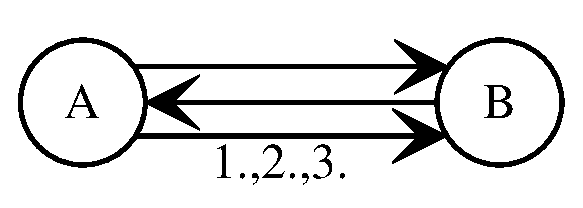
\includegraphics[width=0.5\textwidth]{pic/key_distribution-sts}
    \caption{Взаимодействие участников в протоколе STS\label{fig:key_distribution-sts}}
\end{figure}

\begin{protocol}
    \item[(1)] Алиса выбирает случайное число $R_A: 2 \leq R_A \leq p-1$.
    \item[{}] $Alice \to \left\{ A, m_A = g^{R_A} \bmod p \right\} \to Bob$

    \item[(2)] Боб выбирает случайное число $R_B: 2 \leq R_B \leq p-1$.
    \item[{}] Боб вычисляет сессионный ключ $K = m_A^{R_B} \bmod p$.
    \item[{}] $Bob \to \left\{ B, A, m_B = g^{R_B} \bmod p, E_K( S_B ( m_A, m_B )) \right\} \to Alice$

    \item[(3)] Алиса вычисляет сессионный ключ $K = m_B^{R_A} \bmod p$.
    \item[{}] Алиса проверяет подпись в сообщении $E_K( S_B ( m_A, m_B ))$.
    \item[{}] $Alice \to \left\{ A, B, E_K( S_A ( m_A, m_B ) ) \right\} \to Bob$

    \item[(4)] Боб проверяет подпись в сообщении $E_K( S_A ( m_A, m_B ))$.
\end{protocol}

Протокол обеспечивает гарантию формирования новых ключей (G10), но не совершенную прямую секретность (G9).

Как показала атака Лоу 1996 года (\cite{Lowe:1996}, рис.~\ref{fig:key_distribution-sts-attack}), протокол не может гарантировать аутентификацию субъектов (цель G1), ключей (G7) и подтверждение владения сессионным ключом (G8). Хотя злоумышленник не может получить доступ к новому сессионному ключу, если протокол использовать только для аутентификации субъектов, Алиса может принять злоумышленника за Боба.

\begin{figure}
    \centering
    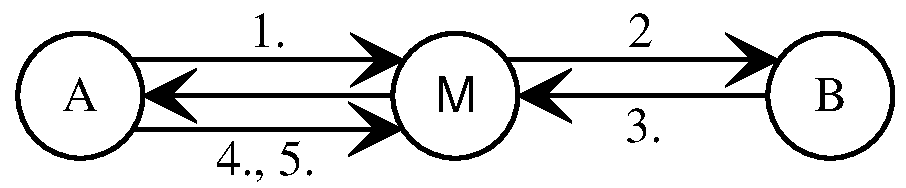
\includegraphics[width=0.67\textwidth]{pic/key_distribution-sts-attack}
    \caption{Схема взаимодействия участников в протоколе STS при атаке Лоу\label{fig:key_distribution-sts-attack}}
\end{figure}

\begin{protocol}
    \item[(1)] Алиса выбирает случайное число $R_A: 2 \leq R_A \leq p-1$.
    \item[{}] $Alice \to \left\{ A, m_A = g^{R_A} \bmod p \right\} \to Mellory~(Bob)$

    \item[(2)] $Mellory~(Alice) \to \left\{ M, m_A \right\} \to Bob$

    \item[(3)] Боб выбирает случайное число $R_B: 2 \leq R_B \leq p-1$ и вычисляет $m_B = g^{R_B} \bmod p$, а также сессионный ключ $K = m_A^{R_B} \bmod p$.
    \item[{}] $Bob \to \left\{ B, M, m_B, E_K( S_B ( m_A, m_B )) \right\} \to Mellory$

    \item[(4)] $Mellory~(Bob) \to \left\{ B, A, m_B, E_K( S_B ( m_A, m_B )) \right\} \to Alice$

    \item[(5)] Алиса вычисляет сессионный ключ $K = m_B^{R_A} \bmod p$.
    \item[{}] Алиса проверяет подпись в сообщении $E_K( S_B ( m_A, m_B ))$.
    \item[{}] $Alice \to \left\{ A, B, E_K( S_A ( m_A, m_B ) ) \right\} \to Mellory~(Bob)$
\end{protocol}

После успешного завершения протокола Алиса уверена, что общается с Бобом.

Как и все остальные <<криптосистемы-протоколы>>, протокол Station-to-Station основывается на некотором внешнем источнике информации об открытых ключах участников, не подвергая сомнению корректность и надёжность этого источника. Что, в общем случае, неверно. Если информацию о ключах участников нужно получать извне при каждом сеансе протокола (например, если участников много, и запомнить ключи всех возможности нет), то канал получения открытых ключей будет основной целью активного криптоаналитика для рассмотренных протоколов. Как от этого защититься с использованием примитивов асимметричной криптографии -- в разделе~\ref{section-protocols-asymmetric}.

\index{протокол!Station-to-Station|)}

\subsection{Схема Жиро}\label{section-girault-scheme}\index{схема!Жиро|(}
\selectlanguage{russian}

В схеме Жиро (\langfr{Marc Girault},~\cite{Girault:1990, Girault:1991}) надёжность строится на стойкости криптосистемы RSA (сложности факторизации больших чисел и вычисления дискретного корня).

Предварительно:
\begin{itemize}
    \item Доверенный центр (Трент, $T$):
    \begin{itemize}
        \item выбирает общий модуль $n = p \times q$, где $p$ и $q$ -- большие простые числа;
        \item выбирает пару из закрытого и открытого ключей $K_{T, \text{public}}: (e, n)$ и $K_{T, \text{private}}: (d, n)$;
        \item выбирает элемент $g$ поля $\mathbb{Z}_n^{\times}$ максимального порядка;
        \item публикует в общедоступном месте параметры схемы $n$, $e$ и $g$.
    \end{itemize}
    \item Каждый из легальных участников:
    \begin{itemize}
        \item выбирает себе закрытый ключ $s_i$ и идентификатор $I_i$;
        \item вычисляет и отправляет доверенному центру $v_i = g^{-s_i} \bmod n$;
        \item используя протокол аутентификации сторон (см. ниже) легальный участник доказывает доверенному центру, что владеет закрытым ключом, не раскрывая его значение;
        \item получает от доверенного центр свой открытый ключ:
            \[ P_i = (v_i - I_i)^d = (g^{-s_i} - I_i)^d \mod n; \]
    \end{itemize}
    В результате для каждого участника, например, Алисы, которая владеет $P_A, I_A, s_a$ будет выполняться утверждение:
        \[ P_A^e + I_A = g^{-s_A} \mod n. \]
\end{itemize}

Протокол аутентификации сторон в общем случае выглядит следующим образом (рис.~\ref{fig:key_distribution-girault-auth}).

\begin{figure}
    \centering
    \includegraphics[width=0.5\textwidth]{pic/key_distribution-girault-auth}
    \caption{Взаимодействия участников в протоколе идентификации Жиро\label{fig:key_distribution-girault-auth}}
\end{figure}

\begin{protocol}
    \item[(1)] Алиса выбирает случайное $R_A$.
    \item[{}] $Alice \to \left\{ I_A, P_A, t = g^{R_A} \right\} \to Bob$
    \item[(2)] Боб выбирает случайное $R_B$.
    \item[{}] $Bob \to \left\{ R_B \right\} \to Alice$
    \item[(3)] $Alice \to \left\{ y = R_A + s_A \times R_B \right\} \to Bob$
    \item[(4)] Боб вычисляет $v_A = P_A^e + I_A$;
    \item[{}] Боб проверяет, что $g^ y v_A^{R_B} = t$.
\end{protocol}

Протокол генерации сессионного ключа, либо просто \emph{схема Жиро}, как и другие схемы, состоит из проходов обмена открытой информацией и вычисления ключа (рис.~\ref{fig:key_distribution-girault-scheme}).

\begin{figure}
    \centering
    \includegraphics[width=0.5\textwidth]{pic/key_distribution-girault-scheme}
    \caption{Взаимодействие участников в схеме Жиро\label{fig:key_distribution-girault-scheme}}
\end{figure}

\begin{protocol}
    \item[(1)] $Alice \to \left\{ P_A, I_A \right\} \to Bob$
    \item[(2)] Боб вычисляет $K_{BA} = (P_A^e + I_A)^{s_B} \bmod n$.
    \item[{}] $Bob \to \left\{ P_B, I_B \right\} \to Alice$
    \item[(3)] Алиса вычисляет $K_{AB} = (P_B^e + I_B)^{s_A} \bmod n$.
\end{protocol}

В результате работы схемы стороны сгенерировали одинаковый общий сеансовый ключ.
\[ K_{AB} = (P_A^e + I_A)^{s_B} = (g^{-s_A})^{s_B} = g^{-s_As_B} \mod n; \]
\[ K_{BA} = (P_B^e + I_B)^{s_A} = (g^{-s_B})^{s_A} = g^{-s_As_B} \mod n; \]
            \[ K = K_{AB} = K_{BA} = g^{-s_As_B} \mod n. \]

Схема обеспечивает аутентификацию ключа (цель G7), так как только легальные пользователи смогут вычислить корректное значение общего сессионного ключа.

\index{схема!Жиро|)}

\subsection{Схема Блома}\index{схема!Блома}
\selectlanguage{russian}

Рассмотрим распределение ключей по \emph{схеме Блома} (Rolf Blom,~\cite{Blom:1984, Blom:1985}), в котором каждые два пользователя из общего числа $N$ пользователей могут создать общий секретный ключ, причём секретные ключи каждой пары различны. Данная схема используется в протоколе HDCP\index{протокол!HDCP} (\langen{High-bandwidth Digital Content Protection}) для предотвращения копирования высококачественного видеосигнала.

На этапе инициализации доверенный центр выбирает симметричную матрицу $D_{m,m}$ над конечным полем $\GF p$. Для присоединения к сети распространения ключей новый участник либо самостоятельно, либо с помощью доверенного центра выбирает новый открытый ключ (идентификатор) $I$, представляющий собой вектор длины $k$ над $\GF p$. Доверенный центр вычисляет для нового участника закрытый ключ $K$:

\begin{equation}
	K = D_{m,m} I.
	\label{eq:blom_center_matrix}
\end{equation}

Симметричность матрицы $D_{m,m}$ доверенного центра позволяет любым двум участникам сети создать общий сеансовый ключ. Пусть Алиса и Боб -- легальные пользователи сети, то есть они обладают открытыми ключами $I_A$ и $I_B$ соответственно, а их закрытые ключи $K_A$ и $K_B$ были вычислены одним и тем же доверенным центром по формуле~\ref{eq:blom_center_matrix}. Тогда протокол выработки общего секретного ключа выглядит следующим образом.

\begin{enumerate}
	\item Алиса отправляет Бобу свой открытый ключ $I_A$.
	\item Боб отправляет Алисе свой открытый ключ $I_B$.
	\item Алиса вычисляет значение $s_{AB} = K^t_A I_B = I^t_A D_{m,m} I_B$.
	\item Боб вычисляет значение $s_{BA} = K^t_B I_A = I^t_B D_{m,m} I_A$.
\end{enumerate}

Из симметричности матрицы $D_{m,m}$ следует, что значения $s_{AB}$ и $s_{BA}$ совпадут, они же и будут являться общим секретным ключом для Алисы и Боба. Этот секретный ключ будет свой для каждой пары легальных пользователей сети.

Присоединение новых участников к схеме строго контролируется доверенным центром, что позволяет защитить сеть от нелегальных пользователей. Надёжность данной схемы основывается на невозможности восстановить исходную матрицу. Однако для восстановления матрицы доверенного центра размера $m \times m$ необходимо и достаточно всего $m$ пар линейно независимых открытых и закрытых ключей. В 2010 году компания Intel, которая является <<доверенным центром>> для пользователей системы защиты HDCP, подтвердила, что криптоаналитикам удалось найти секретную матрицу (точнее, аналогичную ей), используемую для генерации ключей в упомянутой системе предотвращения копирования высококачественного видеосигнала.

